\documentclass[14pt]{extarticle}
\usepackage{fontspec}
\usepackage{polyglossia}
\usepackage{amsmath}
\usepackage{amssymb}
\usepackage{xcolor}
\usepackage{fancyhdr}
\usepackage{graphicx}
\usepackage{listings}
\usepackage[most]{tcolorbox}
% \usepackage{setspace}
\usepackage{pifont}
\usepackage{enumitem}
\usepackage{titlesec}
\usepackage[bottom]{footmisc}
\usepackage{titling}
\usepackage{minted}
\usepackage{etoolbox}
\usepackage{array}
\usepackage{extsizes}
\usepackage{float}
\usepackage{booktabs}
\usepackage{hyperref}
\usepackage[onehalfspacing]{setspace}
\usepackage[a4paper, top=2.7cm, bottom=2.7cm, left=2.5cm, right=2.5cm, headheight=1.5cm, headsep=0.5cm]{geometry}
\usepackage{tikz}

\usetikzlibrary{automata, positioning, arrows.meta, arrows}

\newfontfamily\emoji{Segoe UI Emoji}

\pagestyle{fancy}

\setmainlanguage[numerals=western]{arabic}
\setotherlanguage{english}
% \newfontfamily\arabicfont[Script=Arabic]{Amiri}
\newfontfamily\arabicfont[Script=Arabic]{Calibri}
\newfontfamily\arabicfonttt[Script=Arabic]{Courier New}

\lstset{
  language=[Sharp]C,
  numbers=left,
  stepnumber=1,
  numbersep=8pt,
  frame=single,
  basicstyle=\ttfamily\small,
  keywordstyle=\color{blue},
  stringstyle=\color{red},
  commentstyle=\color{green!50!black}
}

\newif\ifdetailed
\ifdefined\setdetailed
  \setdetailed
\fi

\newif\ifwithsols
\ifdefined\setwithsols
  \setwithsols
\fi

% unified tcolorboxes for articles
\tcbset{colback=white, colframe=black, fonttitle=\bfseries, boxrule=0.8pt}
\newtcolorbox{boxDef}[1][]{colback=blue!5!white,colframe=blue!75!black,
  title={{\emoji📘} تعريف\ifx\\#1\\\else ~#1\fi :}}
\newtcolorbox{boxExercise}[1][]{colback=cyan!5!white,colframe=cyan!70!black,
  title={{\emoji🧩} تمرين\ifx\\#1\\\else ~#1\fi :}}
\newtcolorbox{boxExample}[1][]{colback=yellow!5!white,colframe=orange!90!black,
  title={{\emoji📝} مثال\ifx\\#1\\\else ~#1\fi :}}
\newtcolorbox{boxNote}[1][]{colback=gray!10!white,colframe=black,
  title={{\emoji✨} ملاحظة\ifx\\#1\\\else ~#1\fi :}}
\newtcolorbox{boxAttention}[1][]{colback=magenta!10!white,colframe=magenta!80!black,
  title={{\emoji🔔} تنبيه\ifx\\#1\\\else ~#1\fi :}}
\newtcolorbox{boxWarning}[1][]{colback=red!5!white,colframe=red!75!black,
  title={{\emoji⚡} ملاحظة هامة\ifx\\#1\\\else ~#1\fi :}}
\newtcolorbox{boxSolution}[1][]{colback=green!5!white,colframe=green!60!black,
  title={{\emoji✅} حل\ifx\\#1\\\else ~#1\fi :}}
\newtcolorbox{boxSymbol}[1][]{colback=purple!5!white,colframe=purple!70!black,
  title={{\emoji🔣} رمز\ifx\\#1\\\else ~#1\fi :}}
\newtcolorbox{boxHint}[1][]{colback=teal!5!white,colframe=teal!60!black,
  title={{\emoji💡} تلميح\ifx\\#1\\\else ~#1\fi :}}


\tcbset{simplecode/.style={ colback=gray!5, colframe=black!50, boxrule=0.4pt, arc=2pt, left=4pt,right=4pt,top=4pt,bottom=4pt}}
\newenvironment{boxCode}{\begin{tcolorbox}[simplecode]}{\end{tcolorbox}}

\newcolumntype{C}[1]{>{\centering\arraybackslash}p{#1}}

% redefine spaces after titles
\makeatletter
\renewcommand{\@maketitle}{%
  \begin{center}
    {\huge \bfseries \@title \par}%
    \vskip 0.2em % space between title and author
    {\large \@author \par}%
    % \vskip 0.2em % space between author and date
    % {\normalsize \@date \par}%
  \end{center}
}
\makeatother

\fancyhf{} % clear default
\fancypagestyle{plain}{
  \fancyhf{}
  \fancyhead[L]{مدرسة التسامح الشاملة}
  % \fancyhead[L]{
\includegraphics[height=1cm]{../../../images/logoTasamoh.png}}
  \fancyhead[R]{الأستاذ محمود اغبارية}
  \fancyfoot[C]{\thepage}
}

\fancyhead[L]{مدرسة التسامح الشاملة}
\fancyhead[R]{الأستاذ محمود اغبارية}
\fancyfoot[C]{\thepage}
% \date{\today}

\setcounter{tocdepth}{3} % only section subsection and subsubsection in TOC

\newcommand{\importpdfpage}[2]{%
    \thispagestyle{empty}
    \newgeometry{left=0cm,right=0cm,top=0cm,bottom=0cm}
    \includegraphics[page=#2,width=0.95\paperwidth,height=0.95\paperheight,keepaspectratio]{#1}
    \restoregeometry
}

\newcommand{\insertFullImg}[1]{%
    \noindent
    \makebox[\textwidth][c]{
        \includegraphics[width=0.9\paperwidth,keepaspectratio]{#1}%
    }%
}%

% ----------------------


% \begin{document}

% \maketitle

% % \clearpage  % start TOC on a new page
% % \renewcommand{\contentsname}{جدول المحتويات}
% % \tableofcontents
% % \clearpage

% \part*{part 1} % the * prevents numbering
% \section*{مقدمة}
% \subsection*{مثال رياضي}
% \subsubsection*{مثال فرعي}
% \paragraph*{ paragraph 1}
% \subparagraph*{sub paragraph 1}

% \ifdetailed
% \begin{english}
% \begin{minted}{csharp}
% // C# Example
% \end{minted}
% \end{english}
% \fi

% OLD WAY
% \ifdetailed
% \begin{english}
% \begin{lstlisting}
% // C# Example
% \end{lstlisting}
% \end{english}
% \fi

% % 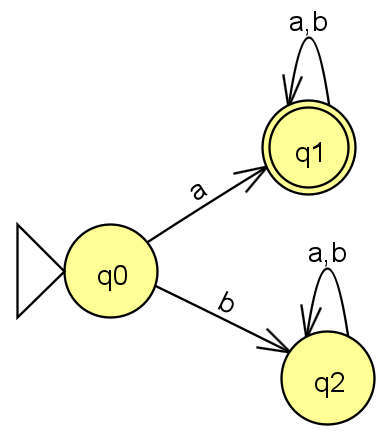
\includegraphics[width=0.2\textwidth]{../../../images/DFAs/ex1_q1.png}



% \vspace{3cm}
% \begin{flushleft}
% أرجو لكم وقتًا ممتعًا.

% الأستاذ محمود اغبارية.
% \end{flushleft}


% \end{document}


\begin{document}

\pagestyle{empty}
\thispagestyle{empty}

\begin{itemize}
    \item \textbf{أوتومات راصة:}
    \begin{enumerate}
        \item
        معطاة اللغة $L$ فوق الأبجدية $\{a, b, c\}$:$$L = \{ a^{2n} b^{n+m} c^{m} \mid n \ge 1, m \ge 1 \}$$أ. (1) ما هي أقصر كلمة تنتمي للغة $L$؟(2) اكتب كلمة تنتمي للغة $L$ طولها 15 حرفًا.ب. ابنِ أوتومات راصة يتلقى اللغة $L$.

        \item
        أمامك اللغتان $L_1$ وَ $L_2$ فوق الأبجدية $\{a, b, c\}$:
        $$L_1 = \{ (ab)^n c^{3m} \mid n \ge 1, m \ge 1 \}$$
        $$L_2 = \{ a^n b^n c^{3m} \mid n \ge 1, m \ge 1 \}$$

        أ. هل اللغة $L_1$ نظاميّة؟ إذا كانت نظاميّة - ابنِ أوتوماتًا نهائيًا محدودًا يتلقى اللغة، وإذا لم تكن نظامية - ابنِ أوتومات راصة يتلقى اللغة. \\
        ب. هل اللغة $L_2$ نظاميّة؟ إذا كانت نظاميّة - ابنِ أوتوماتًا نهائيًا محدودًا يتلقى اللغة، وإذا لم تكن نظامية - ابنِ أوتومات راصة يتلقى اللغة.

        \item
        أمامك اللغة $L$ فوق الأبجدية $\{a, b, c, d\}$:$$L = \{ (ab)^n c^k d^{2n} \mid n \ge 1, k \ge 0, \text{العدد } k \text{ زوجي} \}$$أ. (1) اكتب أقصر كلمة في اللغة $L$.(2) أعطِ مثالاً لكلمة تنتمي للغة $L$ بحيث يكون طولها الإجمالي 10 حروف.ب. ابنِ أوتومات راصة (PDA) يتلقى اللغة $L$.

    \end{enumerate}

\item \textbf{آلة تيورنج:}

    \begin{enumerate}
        \item
اكتبوا آلة تيورنج تتلقى في بداية الشريط عددًا أوناريًا $x$ (أكبر من 0). تعيد الآلة عددًا جديدًا كما هو مفصّل أمامكم:إذا كان العدد المُتلقّى $x$ من مضاعفات العدد 3 (يقبل القسمة على 3 بدون باقٍ)، تعيد الآلة ثلث العدد الأصلي $\frac{x}{3}$.إذا كان العدد المُتلقّى $x$ لا يقبل القسمة على 3، تعيد الآلة شريطًا فارغًا (أي القيمة 0 الأونارية).

\item
آلة تيورنج تتلقى كمدخل كلمة $w$ فوق الأبجدية $\{a, b\}$ مكتوبة من بداية الشريط.
تقوم الآلة بتعديل الكلمة بحيث تُضاعِف كل حرف $a$ (أي تستبدل كل $a$ بـ $aa$) وتترك حرف $b$ كما هو. على سبيل المثال، إذا كانت الكلمة المدخلة هي $w = aab$, فإن الكلمة الناتجة ستكون $w' = aaaab$.

\item
ابنِ آلة تيورنج تتلقى في بداية الشريط عددين صحيحين موجبين $x$ وَ $y$، مسجلين كعددين أوناريّين (بواسطة الرمز 1). تفصل بين العددين الإشارة #.تحسب الآلة الدالة التالية:$$f(x, y) = 2x + y$$يُسجَّل المُخرَج النهائي على الشريط كعدد أوناري بين إشارتي `$$.على سبيل المثال: إذا تلقت الآلة $x=2$ (أي 11) وَ $y=3$ (أي 111)، يجب أن تعيد الآلة القيمة 7 (أي 7 رموز من 1 بين إشارتي $$).توجيهات:لا حاجة للحفاظ على المُدخلات الأصلية (يمكن شطبها أو تغييرها).العدد المُعاد يظهر في مكان ما في الشريط، وباقي الخلايا المجاورة تحتوي على فراغات ($\Delta$).

\item سؤال بناء آلة تيورنج بناء على عملية C#.
\end{enumerate}

\end{itemize}

\end{document}